\documentclass[a4paper,14pt]{extreport}
  \usepackage[left=1.5cm,right=1.5cm,
      top=1.5cm,bottom=2cm,bindingoffset=0cm]{geometry}
  \usepackage{scrextend}
  \usepackage[T1,T2A]{fontenc}
  \usepackage[utf8]{inputenc}
  \usepackage[english,russian,ukrainian]{babel}
  \usepackage{tabularx}
  \linespread{1.3}
  \usepackage[colorinlistoftodos]{todonotes}
  \usepackage{amssymb}
  \usepackage{color}
  \usepackage{amsmath}
  \usepackage{mathrsfs}
  \usepackage{listings}
  \usepackage{graphicx}
  \graphicspath{ {./images/} }
  \usepackage{lipsum}
  \usepackage{xcolor}
  \usepackage{hyperref}
  \usepackage{tcolorbox}

  \usepackage[framemethod=TikZ]{mdframed}
  \usepackage{wrapfig,boxedminipage,lipsum}
  \mdfdefinestyle{MyFrame}{%
  linecolor=blue,outerlinewidth=2pt,roundcorner=20pt,innertopmargin=\baselineskip,innerbottommargin=\baselineskip,innerrightmargin=20pt,innerleftmargin=20pt,backgroundcolor=gray!50!white}
   \usepackage{csvsimple}
   \usepackage{supertabular}
  \usepackage{pdflscape}
  \usepackage{fancyvrb}
  %\usepackage{comment}
  \usepackage{array,tabularx}
  \usepackage{colortbl}

  \usepackage{varwidth}
  \tcbuselibrary{skins}
  \usepackage{fancybox}
  \usepackage{spreadtab}


  \usepackage{tikz}
  \usepackage[framemethod=TikZ]{mdframed}
  \usepackage{xcolor}
  \usetikzlibrary{calc}
  \makeatletter
  \newlength{\mylength}
  \xdef\CircleFactor{1.1}
  \setlength\mylength{\dimexpr\f@size pt}
  \newsavebox{\mybox}
  \newcommand*\circled[2][draw=blue]{\savebox\mybox{\vbox{\vphantom{WL1/}#1}}\setlength\mylength{\dimexpr\CircleFactor\dimexpr\ht\mybox+\dp\mybox\relax\relax}\tikzset{mystyle/.style={circle,#1,minimum height={\mylength}}}
  \tikz[baseline=(char.base)]
  \node[mystyle] (char) {#2};}
  \makeatother
   % Цвета для гиперссылок
  \definecolor{linkcolor}{rgb}{0, 0.72, 0.92} % цвет ссылок
  \definecolor{urlcolor}{rgb}{0.0, 0.0, 1.0}% цвет гиперссылок
  \hypersetup{pdfstartview=FitH,  linkcolor=red,urlcolor=red,citecolor=red, colorlinks=true}

  \definecolor{ggreen}{rgb}{0.4,1,0}
  \definecolor{rred}{rgb}{1,0.1,0.1}
  \definecolor{amber}{rgb}{1.0, 0.75, 0.0}
  \definecolor{babyblue}{rgb}{0.54, 0.81, 0.94}
  \definecolor{amethyst}{rgb}{0.6, 0.4, 0.8}

  \usepackage{float}
  \usepackage{wrapfig}
  \usepackage{framed}
  %for nice Code{
  \lstdefinestyle{customc}{
    belowcaptionskip=1\baselineskip,
    breaklines=true,
    frame=L,
    xleftmargin=\parindent,
    language=C,
    showstringspaces=false,
    basicstyle=\small\ttfamily,
    keywordstyle=\bfseries\color{green!40!black},
    commentstyle=\itshape\color{purple!40!black},
    identifierstyle=\color{blue},
    stringstyle=\color{orange},
  }
  \lstset{escapechar=@,style=customc}
%}


\begin{document}
\renewcommand{\bibname}{Список використаної літератури}% -- переименуем название списка литературы


%указатель -- \cite{lit1}

\pagecolor{white}

%----------------------------------------1
\newtcbox{\xmybox}[1][red]{on line, arc=7pt,colback=#1!10!white,colframe=#1!50!black, before upper={\rule[-3pt]{0pt}{10pt}},boxrule=1pt, boxsep=0pt,left=6pt,right=6pt,top=2pt,bottom=2pt}

\begin{titlepage}
  \begin{center}
  \large
  Національний технічний університет України \\ "Київський політехнічний інститут імені Ігоря Сікорського"


  Факультет Електроніки

  Кафедра мікроелектроніки
  \vfill

  \textsc{РЕФЕРАТ}\\

  %{\Large Про виконання лабораторної роботи №1\\
  з дисципліни: «Фізико - технологічні основи наноелектроніки-2»\\[1cm]

  Фотоприймачі на квантових ямах


  %}
  \bigskip
  \end{center}
  \vfill

  \newlength{\ML}
  \settowidth{\ML}{«\underline{\hspace{0.4cm}}» \underline{\hspace{2cm}}}
  \hfill
  \begin{minipage}{1\textwidth}
  Виконавець:\\
  Студент 4-го курсу \hspace{4cm} $\underset{\text{(підпис)}}{\underline{\hspace{0.2\textwidth}}}$  \hspace{1cm}Грабар О. О.\\
  \vspace{1cm}

  Перевірила: \hspace{5.6cm} $\underset{\text{(підпис)}}{\underline{\hspace{0.2\textwidth}}}$  \hspace{1cm}доц. Орлов В. А.\\

  \end{minipage}

  \vfill

  \begin{center}
  2021
  \end{center}
\end{titlepage}
%\tableofcontents
\setcounter{page}{2}

\newpage


 

%\chapter{ВСТУП}\par
 

Процеси оптичної іонізації квантових ям можуть використовуватися для створення нових типів приймачів інфрачервоного випромінювання. Принцип приймача дуже простий: викид носіїв у зону провідності широкозонного напівпровідника (потенційного бар'єру) збільшує провідність у напрямі, перпендикулярному шарам гетероструктури.\\

За своєю дією такий приймач нагадує домішковий фоторезистор, де у ролі центрів виступають квантові ями. Тому як час життя нерівноважних носіїв виступає характерний час захоплення квантову яму $\tau q$. Порівняно із звичайним часом життя, пов'язаним із захопленням на рекомбінаційні центри, $\tau q$ має дві важливі відмінності.\\

По-перше, $\tau q$ значно (на кілька порядків) менше часу захвату на центри. Причина в тому, що акт захоплення пов'язаний з необхідністю передачі решітці від носія досить великої енергії, що дорівнює енергії зв'язку центру або величині $\triangle$E при захопленні в квантову яму. Найбільш ефективний механізм передачі енергії - це випромінювання оптичних фотонів з енергією $hw_0$/2p. Однак енергія зв'язку центрів аж ніяк не збігається з $hw_0$/2p і тому такий процес неможливий. Електрон повинен віддавати енергію в ході значно повільнішого каскадного процесу випромінювання багатьох акустичних фононів. У разі квантової ями наявність безперервного діапазону руху в площині ями значно змінює ситуацію. Стає можливим перехід на пов'язаний стан у ямі при випромінюванні оптичного фонону з одночасною передачею надлишкової енергії, що залишилася, в рух у площині ями (рисунок 8). Якщо вихідний електрон мав енергію, близьку до краю зони в широкозонному матеріалі, то з малюнка 8 видно, що фонон, що випускається, повинен мати досить великий імпульс:\\
\[ q = [2m (\triangle E - E1 - h\omega_0/2\pi)]^{1/2}\]
у площині квантової ями. Значно більша величина
взаємодії електронів з оптичними фононами, ніж з
акустичними, визначає трохи $\tau q$ в порівнянні з часом
захоплення із центру.\\ 

По-друге, $\tau q$ немонотонним, осцилюючим чином залежить
параметрів ями. Це з властивостями хвильової функції електронів у делокализованных станах над квантової ямою $\psi_{\pounds}$.
Якщо яма не є резонансною, то амплітуда цієї хвильової
функції у безпосередній околиці ями при малій енергії
електрона дуже мала. Власне, $\tau q$ буде відносно велике. Для
резонансних квантових ям ймовірність захоплення зростає, тобто $\tau q$
падає.\\ 

Фотопровідність аналізованої структури, як і
звичайного фоторезистора, визначається добутком трьох факторів:
швидкості оптичної генерації, яка у свою чергу
пропорційна коефіцієнту поглинання $\alpha$, часу життя в
справакалізованому стані $\tau q$ та ефективної рухливості в ньому $\mu_{\text{еф}}$,
яка має бути пропорційна квантово-механічному
коефіцієнт проходження електрона над квантовою ямою. Перший і
треті фактори максимальні для резонансних квантових ям, а $\tau q$,
навпаки, мінімально їм. Однак сукупна дія всіх
факторів виявляється таким, що фотоприймачі на квантових
ямах матимуть найкращі параметри у разі резонансних ям.\\ 

\begin{figure}[h!]
   \center{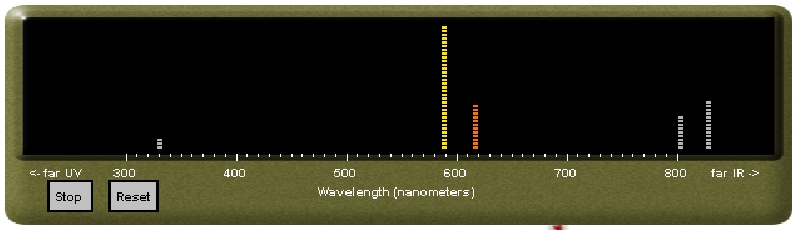
\includegraphics[width=0.5\linewidth]{3.png}}
   \caption{Процес захоплення нерівноважного електрона у квантову
яму з випромінюванням оптичного фонону.}
   \label{r3}
 \end{figure}

 Приймачі на основі квантових ям можуть скласти
конкуренцію фоточутливим структурам на основі твердих
розчинів CdHgTe - найважливішого типу приймачів для цього
спектрального діапазону Основною перевагою структур на
квантових ямах є більша стабільність і менший розкид
параметрів, що особливо важливо для матричних фоточутливих
структур.\\ 

Шляхом порівняно невеликих змін складу
широкозонних шарів та товщини ями можна змінювати положення
максимуму та ширину смуги фоточутливості. Останнє
обставина пов'язана з тим, що в міру порушення точної умови
Резонанс спектр фотоіонізації квантової ями стає більш
плавним та має менш різкий максимум.\\ 

\begin{figure}[h!]
   \center{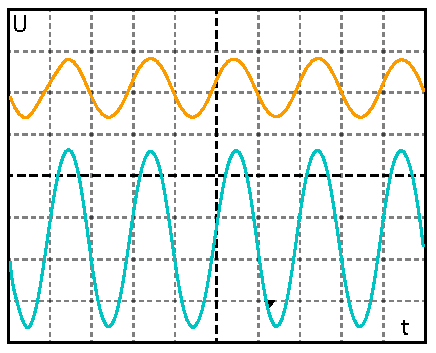
\includegraphics[width=0.7\linewidth]{4.png}}
   \caption{Способи введення випромінювання у фотоприймач з
квантовими ямами: а - через скошений торець підкладки,
б - за допомогою дифракційної решітки;
1 - підкладка, 2 - фоточутлива структура з
квантовими ямами, 3-дифракційні грати.}
   \label{r4}
 \end{figure}

У зв'язку з тим, що оптична іонізація квантових ям може
викликатись лише світлом, поляризованим за нормаллю до квантових
шарам, описані фотоприймачі повинні містити спеціальні
пристосування, що поляризують падаюче світло необхідним чином.
Є два основні способи зробити це. Світло може прямувати в
фоточутливу структуру під кутом через скошений торець
підкладки (Рис. \ref{r4} a). В іншому варіанті світло проходить через
підкладку за нормаллю, а належну поляризацію набуває після
дифракції на решітці, спеціально нанесеній на верхню
поверхню структури (Рис. \ref{r4} б).\\

Можливе альтернативне вирішення проблеми поляризації,
що дозволяє уникнути описаних вище конструкційних
ускладнень. Йдеться про вирощування квантових структур з
напівпровідників з анізотропним енергетичним спектром При
наявності анізотропії електричне поле нормально падаючої
світлової хвилі, що лежить у площині шарів, надає електронам
імпульс під деяким кутом до цієї поверхні. З позицій квантової
механіки це означає можливість переходів між різними
квантово-розмірними рівнями або між рівнем та континуумом
станів над квантовою ямою, що потрібно для роботи приймача.
На практиці для реалізації цієї ідеї найчастіше використовують
гетероструктури на основі тієї ж, найбільш освоєної
технологічно, системи $GaAs-Al_xGa_{1-x}As$, але мають не n-, а p-тип
легування. При цьому складний характер енергетичного спектру
валентної зони забезпечує фоточутливість при нормальному
падіння світла.


%==================================          KPI KNIGA                =========================

Середній інфрачервоний (ІЧ) діапазон (3–50 мкм) цікавий з точки
зору контролю технологічних процесів, екологічного моніторингу,
лазерного зв’язку (особливо – космічного), виявлення та ідентифікації
цілей, спектроскопії, астрономії та медичної діагностики. У цьому
діапазоні можуть працювати фотоприймачі на основі напівпровідників
з малою шириною забороненої зони.\\ 
 
Можна зауважити, що в науково-технічній літературі (і навіть в
стандартах) немає одностайності відносно меж ближнього, середнього
та дальнього ІЧ діапазонів. У навчальному посібнику вказані межі
діапазонів, які майже точно відповідають стандарту ISO 20473: 0,8–
3,0 мкм – ближній ІЧ (англ. near-infrared, NIR), 3–50 мкм – середній ІЧ
(mid-infrared, MIR), 50–1000 мкм – дальній ІЧ (far-infrared, FIR). Автор
лише замінив межу 1000 мкм на 2000 мкм, оскільки за довгохвильовою
межею стандарту у деяких молекул є ще спектральні лінії, на яких
можна отримати оптичне міліметрове випромінювання оптичними
методами (наприклад, збудженням молекул води або кисню
випромінюванням $CO_2$-лазера). \\ 

Недоліком гомо- та гетероперехідних фотоприймачів, в яких
фотоелектричний ефект виникає внаслідок міжзонних переходів
електронів, є обмеження швидкодії паразитною ємністю p–n-переходів.
Можливість отримати фотоелектричний ефект на основі внутрізонних
переходів значно підвищила б швидкодію фотоприймачів. Така
можливість була реалізована у фотоприймачі на квантових ямах,
створеному у 1987 р. американським фізиком Левіним Б. Ф. зі
співробітниками. Автори назвали розроблений прилад
«інфрачервоний фотоприймач на квантових ямах» (англ. quantum well
infrared photodetector, QWIP). Розгляньмо принцип дії такого
фотоприймача.\\ 

Фотоприймач містить від 20 до 50 квантових ям, розділених
бар’єрами. Ширину квантових ям роблять такою, щоб всередині ями
електрони могли знаходитись лише у двох станах – основному (біля
дна зони провідності ями) та збудженому (біля дна зони провідності
бар’єру). Бар’єри значно ширші за ями, що унеможливлює квантове
тунелювання електронів між ямами. Якщо квантові ями створюють з
 GaAs, то бар’єри – з AlGaAs, причому GaAs легують донорною
домішкою, щоб основний стан зони провідності був заповнений
електронами.\\ 

На рис. \ref{r1}  зображені зона провідності QWIP (для спрощення – з
двома квантовими ямами) та процес формування у приймачі
фотоструму. Нахил дна зони провідності виникає внаслідок
прикладення до структури зовнішнього електричного поля Е (напруги
між колектором та емітером). Світло вивільняє електрони з квантових
ям, а електричне поле переносить електрони вздовж надрешітки, від
емітера до колектора, підсилюючи фотострум внаслідок ударної
іонізації (як у фоторезисторі).

\begin{figure}[h!]
   \center{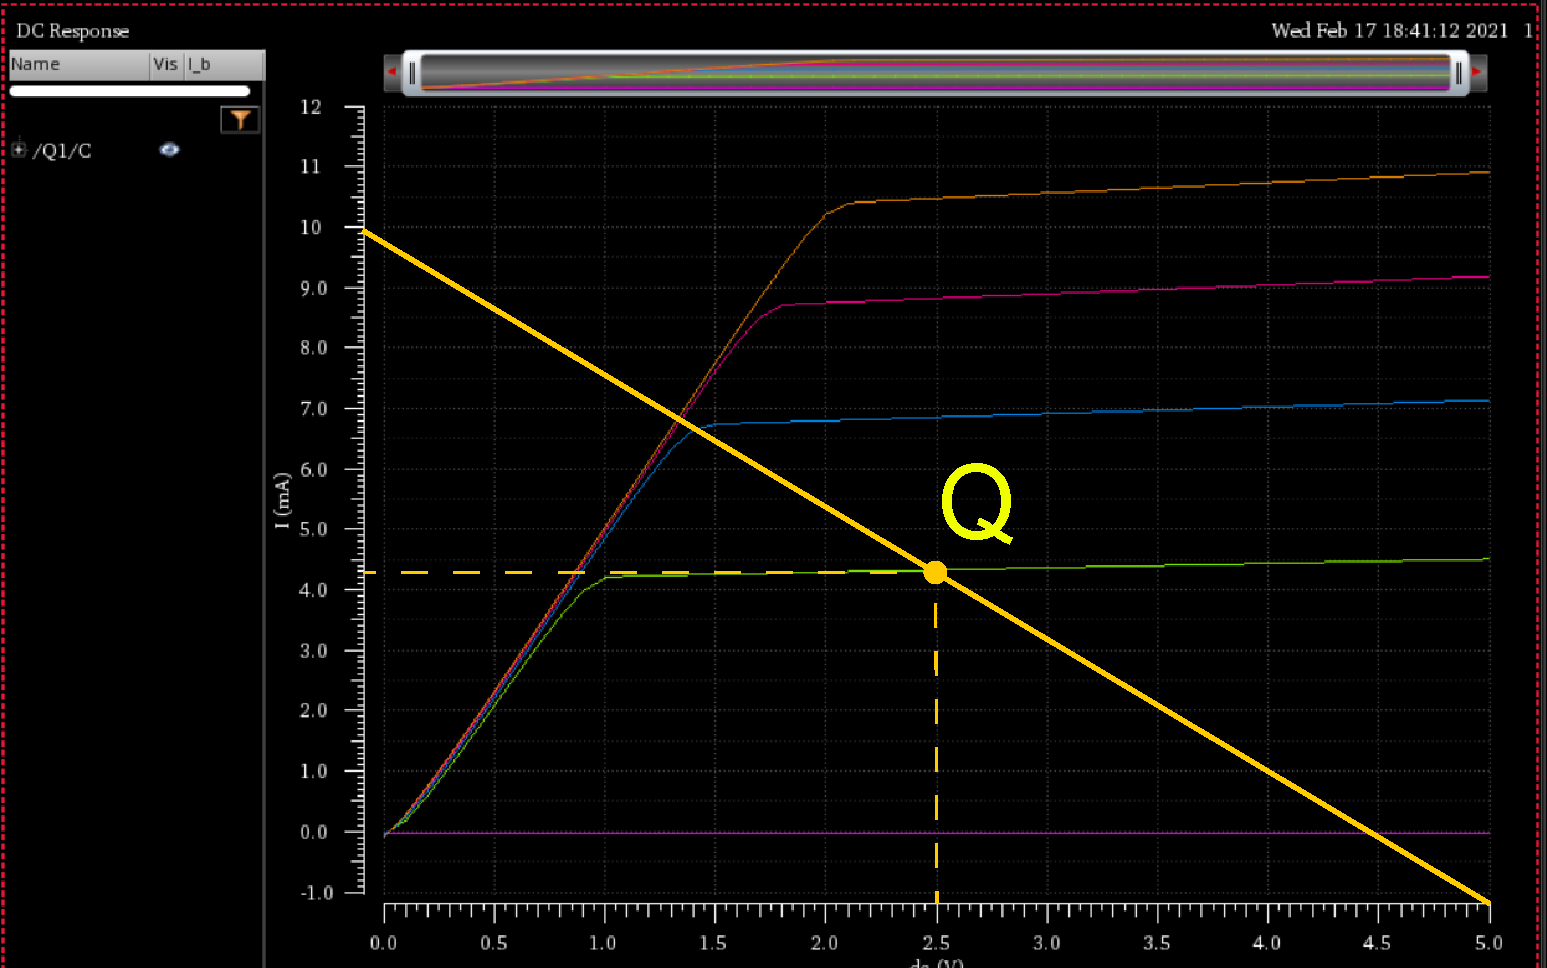
\includegraphics[width=0.9\linewidth]{1.png}}
   \caption{Схема формування та підсилення фотоструму в QWIP}
   \label{r1}
 \end{figure}
Таким чином, QWIP працює у фотопровідному режимі із прикладеним
зовнішнім електричним полем і за відсутності освітлення по ньому
протікає темновий струм.\\ 

Іншим приладом на внутрізонних переходах, до того ж з
убудованим електричним полем, став квантово-каскадний
фотоприймач (англ. quantum cascade detector, QCD). Цей прилад
працює у фотогальванічному режимі і не має темнового струму.
Розгляньмо принцип дії такого приладу (рис. \ref{r2}).\\ 

Надрешітка квантово-каскадного фотоприймача зазвичай налічує
20–40 періодів. Один період складається з поглинальної квантової ями
А і екстракторного каскаду ям B–H, відповідального за перенесення
електронів від одного періоду до іншого. Квантова яма А утворена
напівпровідником, виродженим за електронами, так що рівень Фермі
для електронів лежить вище основного рівня зони провідності.
Квантові ями B–H створені нелегованим напівпровідником, причому їх
ширина поступово зростає, а ширина квантових бар’єрів між ними
зменшується, так що період надрешітки поступово зростає. Завдяки
цьому виникає внутрішнє електричне поле, яке екстрагує електрони з
ями А і переносить їх на основний рівень ями А' наступного періоду 
надрешітки. Перенесення електронів від ями до ями формує зрештою
фотострум квантово-каскадного фотоприймача.\\ 

\begin{figure}[h!]
   \center{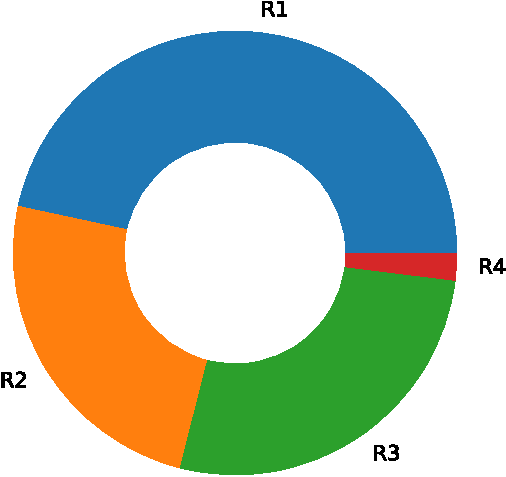
\includegraphics[width=0.9\linewidth]{2.png}}
   \caption{Профіль зони провідності квантово-каскадного фотоприймача
з поглинальною квантовою ямою А та каскадом екстракторних ям В–H}
   \label{r2}
 \end{figure}

Поглинувши енергію фотона, електрон переходить у квантовій ямі
з основного рівня (найнижчого рівня зони провідності) на один з
верхніх енергетичних рівнів, які утворюють мінізону. Нерівноважний
електрон екстрагується з першої квантової ями надрешіткою з плавно
зростаючим періодом і переноситься надрешіткою у другий період, на
основний рівень другої квантової ями.\\ 

Квантово-каскадні фотоприймачі виготовляють з таких пар
матеріалів (яма–бар’єр), як InGaAs–InAlAs, InGaAs–AlAsSb та GaAs–
AlGaAs. На останній парі створені фотоприймачі, які за температури
10 К мають на $\lambda$ = 87 мкм чутливість 8,6 мА/Вт.


























%==================================          KPI KNIGA        END        =========================

 






\begin{thebibliography}{9}
\bibitem{lit1}   Ч. Пулл - мол., Ф. Оуенс Мир матеріалів і технологій, Москва .: Техносфера, 2006. - 336 с.
\bibitem{lit2}  Парфьонов В.В., Закіров Р.Х., Болтакова Н.В. Фізика напівпровідникових приладів: методич. посібник до практикуму з фізики твердого тіла. Казань: Изд-во КДУ, 2004. - 54с.
\bibitem{lit3}  У. Хартманн. Очарование нанотехнологии. – Издательство: Бином,
2008. – 173 с. 
\bibitem{lit4} Ю.А. Чаплыгина. Нанотехнологии в электронике. – Издательство:
Техносфера, 2005. – 448 с.

\end{thebibliography}
\end{document}
